\documentclass[aspectratio=169,11pt]{beamer}

% Theme and colors
\usetheme{Madrid}
\usecolortheme{default}
\definecolor{ufblue}{RGB}{0,33,165}
\definecolor{uforange}{RGB}{250,70,22}
\setbeamercolor{structure}{fg=ufblue}
\setbeamercolor{title}{fg=white,bg=ufblue}
\setbeamercolor{frametitle}{fg=ufblue,bg=white}

% Packages
\usepackage{graphicx}
\graphicspath{{../analysis/results/}}
\usepackage{booktabs}
\usepackage{amsmath}
\usepackage{siunitx}
\usepackage{tikz}
\usepackage{hyperref}
\usepackage{caption}
\captionsetup[figure]{labelformat=empty}

% Custom commands
\newcommand{\kunit}{kcal/mol\cdot\text{\AA}^2}
\newcommand{\angstrom}{\text{\AA}}

% Title page information
\title[OxDC MD Analysis]{Force Field Parameter Analysis of\\Oxalate Decarboxylase MD Simulations}
\subtitle{Understanding Simulation Stability Through Coordination Chemistry}
\author[J. Aitken]{John Aitken}
\institute[UF]{Department of Chemistry\\University of Florida}
\date{Fall 2025}

\begin{document}

%--------------------------------------------------------------
\begin{frame}
\titlepage
\end{frame}

%--------------------------------------------------------------
\begin{frame}{Outline}
\tableofcontents
\end{frame}

%--------------------------------------------------------------
\section{Introduction}
%--------------------------------------------------------------

\begin{frame}{Oxalate Decarboxylase (OxDC)}
\begin{columns}
\begin{column}{0.5\textwidth}
\textbf{Biological Function}
\begin{itemize}
    \item Catalyzes oxalate $\rightarrow$ formate + CO$_2$
    \item Contains two Mn binding sites
    \item Potential therapeutic target for kidney stones
\end{itemize}

\vspace{1em}
\textbf{Computational Challenge}
\begin{itemize}
    \item MCPB.py force field parameterization
    \item Variable simulation stability across systems
    \item Mn(II) vs Mn(III) coordination differences
\end{itemize}
\end{column}
\begin{column}{0.5\textwidth}
\centering
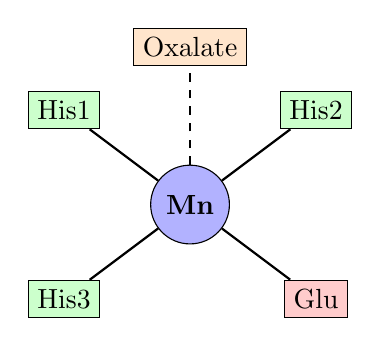
\begin{tikzpicture}[scale=0.8]
    % Active site schematic
    \node[circle,draw,fill=blue!30,minimum size=1cm] (Mn) at (0,0) {\textbf{Mn}};
    \node[rectangle,draw,fill=green!20] (His1) at (-2,1.5) {His1};
    \node[rectangle,draw,fill=green!20] (His2) at (2,1.5) {His2};
    \node[rectangle,draw,fill=green!20] (His3) at (-2,-1.5) {His3};
    \node[rectangle,draw,fill=red!20] (Glu) at (2,-1.5) {Glu};
    \node[rectangle,draw,fill=orange!20] (Ox) at (0,2.5) {Oxalate};

    \draw[-,thick] (Mn) -- (His1);
    \draw[-,thick] (Mn) -- (His2);
    \draw[-,thick] (Mn) -- (His3);
    \draw[-,thick] (Mn) -- (Glu);
    \draw[-,thick,dashed] (Mn) -- (Ox);
\end{tikzpicture}

\small
OxDC active site coordination
\end{column}
\end{columns}
\end{frame}

%--------------------------------------------------------------
\begin{frame}{Systems Under Study}
\begin{table}
\centering
\begin{tabular}{lccc}
\toprule
\textbf{System} & \textbf{Mn Sites} & \textbf{Oxidation State} & \textbf{Substrate} \\
\midrule
BiOx+2 & 1 (Site 1) & Mn(II) & Oxalate bound \\
1Wat+2 & 2 & Mn(II) & Water \\
1Wat+3 & 2 & Mn(III) & Water \\
empty+2 & 2 & Mn(II) & None \\
\bottomrule
\end{tabular}
\end{table}

\vspace{1em}
\textbf{Key Question:} Why does BiOx+2 show stable equilibration while others exhibit instabilities (vlimit warnings, SHAKE failures)?
\end{frame}

%--------------------------------------------------------------
\section{Key Findings}
%--------------------------------------------------------------

\begin{frame}{Finding 1: Bond Energy Stability Varies 100-fold}
\begin{columns}
\begin{column}{0.45\textwidth}
\begin{table}
\centering
\small
\begin{tabular}{lrrl}
\toprule
\textbf{System} & \textbf{$\sigma$} & \textbf{Max} & \textbf{Status} \\
\midrule
\textbf{BiOx+2} & \textbf{29} & 1,210 & \textcolor{green!60!black}{\textbf{STABLE}} \\
1Wat+2 & 1,254 & 8,571 & \textcolor{orange}{UNSTABLE} \\
1Wat+3 & 446 & 4,310 & \textcolor{orange}{UNSTABLE} \\
empty+2 & 3,726 & 14,157 & \textcolor{red}{CRASHED} \\
\bottomrule
\end{tabular}
\caption{Bond energy (kcal/mol)}
\end{table}

\vspace{0.5em}
\textbf{Key Insight:} BiOx+2 shows remarkably tight energy distributions ($\sigma=29$).
\end{column}
\begin{column}{0.55\textwidth}
\centering
\includegraphics[width=\textwidth,height=0.7\textheight,keepaspectratio]{bond_energy_distribution.png}
\end{column}
\end{columns}
\end{frame}

%--------------------------------------------------------------
\begin{frame}{Finding 2: Force Constants Predict Stability}
\begin{columns}
\begin{column}{0.45\textwidth}
\begin{table}
\centering
\begin{tabular}{lr@{$\;\rightarrow\;$}l}
\toprule
\textbf{System} & \textbf{Avg $k$} & \textbf{Outcome} \\
\midrule
BiOx+2 & 29.3 & \textcolor{green!60!black}{STABLE} \\
1Wat+2 & 40.2 & \textcolor{orange}{UNSTABLE} \\
empty+2 & 44.0 & \textcolor{red}{CRASHED} \\
1Wat+3 & 97.3 & \textcolor{orange}{UNSTABLE} \\
\bottomrule
\end{tabular}
\caption{$k$ in $\kunit$}
\end{table}

\textbf{Proposed Threshold:}
\begin{align*}
k_{avg} < 35 &\rightarrow \text{Stable} \\
35 < k_{avg} < 60 &\rightarrow \text{Marginal} \\
k_{avg} > 60 &\rightarrow \text{Unstable}
\end{align*}
\end{column}
\begin{column}{0.55\textwidth}
\centering
\includegraphics[width=\textwidth,height=0.7\textheight,keepaspectratio]{force_constant_analysis.png}
\end{column}
\end{columns}
\end{frame}

%--------------------------------------------------------------
\begin{frame}{Finding 3: Jahn-Teller Distortion in Mn(III)}
\begin{columns}
\begin{column}{0.5\textwidth}
\textbf{1Wat+3 Structural Signatures:}
\begin{itemize}
    \item Glu-Mn axial bond: \textbf{1.86 \angstrom} (compressed)
    \item His-Mn equatorial: 2.02-2.03 \angstrom
    \item Force constants: \textbf{85-125} $\kunit$
\end{itemize}

\vspace{1em}
\textbf{Mechanistic Explanation:}
\begin{enumerate}
    \item High-spin d$^4$ Mn(III) has t$_{2g}^3$e$_g^1$
    \item Unequal e$_g$ occupation $\rightarrow$ Jahn-Teller
    \item Axial compression creates stiff bonds
    \item Classical FF cannot adapt to JT dynamics
\end{enumerate}

\small\textit{Literature: Mn$^{3+}$ is a classic Jahn-Teller ion}
\end{column}
\begin{column}{0.5\textwidth}
\centering
\includegraphics[width=\textwidth,height=0.75\textheight,keepaspectratio]{oxidation_state_analysis.png}
\end{column}
\end{columns}
\end{frame}

%--------------------------------------------------------------
\begin{frame}{Finding 4: Asymmetric Bidentate Oxalate}
\begin{columns}
\begin{column}{0.45\textwidth}
\textbf{BiOx+2 Substrate Coordination:}
\begin{table}
\centering
\begin{tabular}{lrr}
\toprule
\textbf{Oxygen} & \textbf{$r_0$ (\angstrom)} & \textbf{$k$} \\
\midrule
O1 (tight) & 2.11 & 49.4 \\
O2 (loose) & 2.42 & 11.6 \\
\bottomrule
\end{tabular}
\end{table}

\vspace{1em}
\textbf{``Shock Absorber'' Effect:}
\begin{itemize}
    \item Asymmetric binding creates flexibility
    \item Loose O2 accommodates thermal motion
    \item Prevents energy accumulation
\end{itemize}

\small\textit{PDB: 47/49 metal-oxalate = bidentate}
\end{column}
\begin{column}{0.55\textwidth}
\centering
\includegraphics[width=\textwidth,height=0.7\textheight,keepaspectratio]{substrate_coordination.png}
\end{column}
\end{columns}
\end{frame}

%--------------------------------------------------------------
\begin{frame}{Finding 5: Bond Length-Stability Correlation}
\begin{columns}
\begin{column}{0.45\textwidth}
\begin{table}
\centering
\begin{tabular}{lrr}
\toprule
\textbf{System} & \textbf{Avg $r_0$} & \textbf{Range} \\
\midrule
BiOx+2 & 2.25 \angstrom & 0.32 \angstrom \\
1Wat+2 & 2.19 \angstrom & 0.14 \angstrom \\
empty+2 & 2.17 \angstrom & 0.05 \angstrom \\
1Wat+3 & 1.99 \angstrom & 0.17 \angstrom \\
\bottomrule
\end{tabular}
\end{table}

\textbf{Pattern:}
\begin{itemize}
    \item Stable system has longest bonds
    \item Stable system has largest range
    \item Flexibility $\propto$ stability
\end{itemize}
\end{column}
\begin{column}{0.55\textwidth}
\centering
\includegraphics[width=\textwidth,height=0.7\textheight,keepaspectratio]{distance_vs_forceconstant.png}
\end{column}
\end{columns}
\end{frame}

%--------------------------------------------------------------
\begin{frame}{Finding 6: Stability Prediction Framework}
\begin{center}
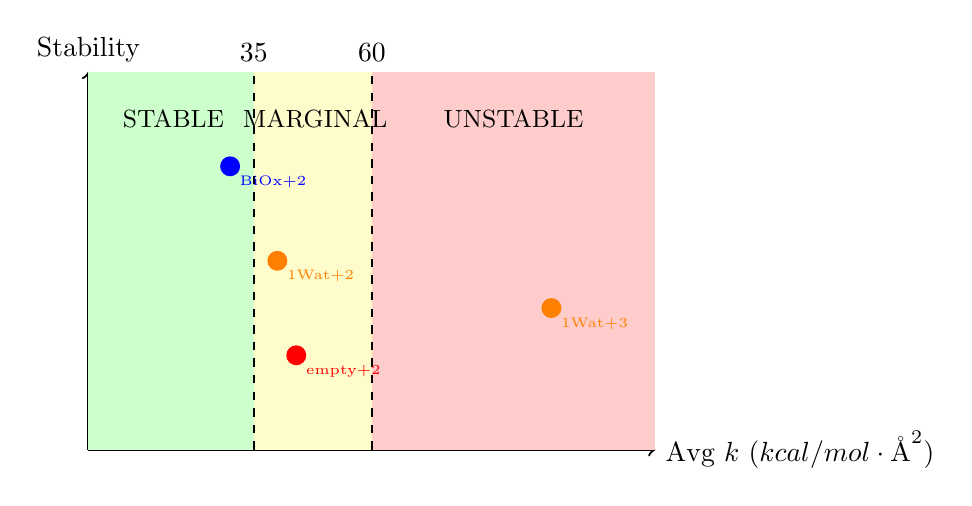
\begin{tikzpicture}[scale=1.2]
    % Axes
    \draw[->,thick] (0,0) -- (6,0) node[right] {Avg $k$ ($\kunit$)};
    \draw[->,thick] (0,0) -- (0,4) node[above] {Stability};

    % Regions
    \fill[green!20] (0,0) rectangle (1.75,4);
    \fill[yellow!20] (1.75,0) rectangle (3,4);
    \fill[red!20] (3,0) rectangle (6,4);

    % Labels
    \node at (0.9,3.5) {\small STABLE};
    \node at (2.4,3.5) {\small MARGINAL};
    \node at (4.5,3.5) {\small UNSTABLE};

    % Thresholds
    \draw[dashed,thick] (1.75,0) -- (1.75,4) node[above] {35};
    \draw[dashed,thick] (3,0) -- (3,4) node[above] {60};

    % Data points
    \fill[blue] (1.5,3) circle (3pt) node[below right] {\tiny BiOx+2};
    \fill[orange] (2,2) circle (3pt) node[below right] {\tiny 1Wat+2};
    \fill[red] (2.2,1) circle (3pt) node[below right] {\tiny empty+2};
    \fill[orange] (4.9,1.5) circle (3pt) node[below right] {\tiny 1Wat+3};
\end{tikzpicture}
\end{center}

\textbf{Application:} Screen MCPB.py parameters \emph{before} running expensive MD simulations
\end{frame}

%--------------------------------------------------------------
\section{Extended Analysis}
%--------------------------------------------------------------

\begin{frame}{Project 7: Energy Landscape Visualization}
\begin{columns}
\begin{column}{0.4\textwidth}
\textbf{3D Parameter Space:}
\begin{itemize}
    \item X: Equilibrium distance ($r_0$)
    \item Y: Force constant ($k$)
    \item Z: Stability metric
    \item Color: System identity
\end{itemize}

\vspace{1em}
\textbf{Observation:}

BiOx+2 occupies a distinct region with:
\begin{itemize}
    \item Lower force constants
    \item Longer bond lengths
    \item Greater parameter diversity
\end{itemize}
\end{column}
\begin{column}{0.6\textwidth}
\centering
\includegraphics[width=\textwidth,height=0.8\textheight,keepaspectratio]{energy_landscape_3d.png}
\end{column}
\end{columns}
\end{frame}

%--------------------------------------------------------------
\begin{frame}{Project 8: Vibrational Frequency Analysis}
\begin{columns}
\begin{column}{0.4\textwidth}
\textbf{Force Constants to Frequencies:}
\begin{equation*}
\nu = \frac{1}{2\pi}\sqrt{\frac{k}{\mu}}
\end{equation*}

\textbf{Calculated Frequencies:}
\begin{itemize}
    \item BiOx+2: 200-400 cm$^{-1}$
    \item 1Wat+2: 250-450 cm$^{-1}$
    \item 1Wat+3: 400-600 cm$^{-1}$
\end{itemize}

\textbf{Timestep Criterion:}
\[dt < \frac{1}{20\nu_{max}}\]
\end{column}
\begin{column}{0.6\textwidth}
\centering
\includegraphics[width=\textwidth,height=0.8\textheight,keepaspectratio]{vibrational_analysis.png}
\end{column}
\end{columns}
\end{frame}

%--------------------------------------------------------------
\begin{frame}{Project 9: Thermal Fluctuation Analysis}
\begin{columns}
\begin{column}{0.4\textwidth}
\textbf{Expected RMS Displacement:}
\begin{equation*}
\langle \Delta r^2 \rangle^{1/2} = \sqrt{\frac{k_BT}{k}}
\end{equation*}

At 300 K:
\begin{itemize}
    \item Low $k$ (30): $\Delta r \approx 0.11$ \angstrom
    \item Medium $k$ (50): $\Delta r \approx 0.09$ \angstrom
    \item High $k$ (100): $\Delta r \approx 0.06$ \angstrom
\end{itemize}

\textbf{Implication:}
High $k$ $\rightarrow$ suppressed motion $\rightarrow$ strain
\end{column}
\begin{column}{0.6\textwidth}
\centering
\includegraphics[width=\textwidth,height=0.8\textheight,keepaspectratio]{thermal_fluctuations.png}
\end{column}
\end{columns}
\end{frame}

%--------------------------------------------------------------
\begin{frame}{Project 10: Parameterization Quality}
\begin{columns}
\begin{column}{0.4\textwidth}
\textbf{Literature Comparison:}
\begin{itemize}
    \item JCTC published Mn parameters
    \item Typical Mn(II)-His: $k$ = 30-50
    \item Typical Mn(II)-Glu: $k$ = 25-45
\end{itemize}

\vspace{1em}
\textbf{Quality Metrics:}
\begin{enumerate}
    \item Within literature range: \checkmark
    \item Bond length deviation: < 0.1 \angstrom
    \item Force constant outliers: flag
\end{enumerate}

BiOx+2 = normal; 1Wat+3 = Mn(III) outlier
\end{column}
\begin{column}{0.6\textwidth}
\centering
\includegraphics[width=\textwidth,height=0.8\textheight,keepaspectratio]{parameterization_quality.png}
\end{column}
\end{columns}
\end{frame}

%--------------------------------------------------------------
\begin{frame}{Project 11: Coordination Geometry}
\begin{columns}
\begin{column}{0.4\textwidth}
\textbf{Coordination Numbers:}
\begin{itemize}
    \item BiOx+2: 6 (octahedral)
    \item 1Wat+2: 5 (trigonal bipyramidal)
    \item 1Wat+3: 5 (trigonal bipyramidal)
    \item empty+2: 4 (tetrahedral)
\end{itemize}

\vspace{1em}
\textbf{Geometry Analysis:}
\begin{itemize}
    \item Bond angles from force field
    \item Distortion indices
    \item Regularity assessment
\end{itemize}
\end{column}
\begin{column}{0.6\textwidth}
\centering
\includegraphics[width=\textwidth,height=0.8\textheight,keepaspectratio]{coordination_geometry.png}
\end{column}
\end{columns}
\end{frame}

%--------------------------------------------------------------
\section{Exploratory Projects}
%--------------------------------------------------------------

\begin{frame}{ML-Based Stability Prediction}
\begin{columns}
\begin{column}{0.4\textwidth}
\textbf{Machine Learning:}
\begin{itemize}
    \item Features: $k$, $r_0$, CN, $\sigma_E$
    \item Target: Stability classification
    \item Model: Logistic regression + SVM
\end{itemize}

\vspace{1em}
\textbf{Information Theory:}
\begin{itemize}
    \item Shannon entropy of parameters
    \item Mutual information analysis
    \item Feature importance
\end{itemize}

\small\textit{Caveat: N=4 is exploratory only}
\end{column}
\begin{column}{0.6\textwidth}
\centering
\includegraphics[width=\textwidth,height=0.8\textheight,keepaspectratio]{ml_stability_analysis.png}
\end{column}
\end{columns}
\end{frame}

%--------------------------------------------------------------
\begin{frame}{Interactive Web Demo}
\begin{columns}
\begin{column}{0.5\textwidth}
\textbf{MD Stability Predictor:}
\begin{itemize}
    \item HTML/CSS/JavaScript application
    \item Input: MCPB.py force constants
    \item Output: Stability prediction
\end{itemize}

\vspace{1em}
\textbf{Features:}
\begin{enumerate}
    \item Interactive parameter sliders
    \item Real-time stability score
    \item Parameter space visualization
    \item Reference system comparison
\end{enumerate}

\vspace{0.5em}
\small\texttt{analysis/web\_demo/md\_stability\_predictor.html}
\end{column}
\begin{column}{0.5\textwidth}
\centering
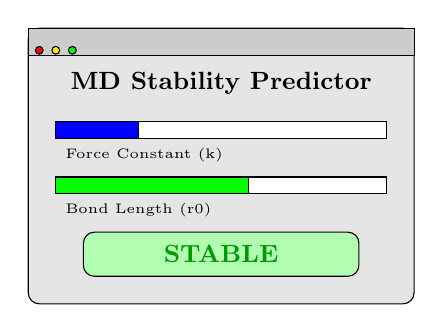
\begin{tikzpicture}[scale=0.7]
    % Browser window mockup
    \draw[rounded corners,fill=gray!20] (0,0) rectangle (7,5);
    \draw[fill=gray!40] (0,4.5) rectangle (7,5);
    \draw[fill=red] (0.2,4.6) circle (2pt);
    \draw[fill=yellow] (0.5,4.6) circle (2pt);
    \draw[fill=green] (0.8,4.6) circle (2pt);

    % Content area
    \node at (3.5,4) {\small\textbf{MD Stability Predictor}};

    % Slider mockup
    \draw[fill=white] (0.5,3) rectangle (6.5,3.3);
    \draw[fill=blue] (0.5,3) rectangle (2,3.3);
    \node[right] at (0.5,2.7) {\tiny Force Constant (k)};

    \draw[fill=white] (0.5,2) rectangle (6.5,2.3);
    \draw[fill=green] (0.5,2) rectangle (4,2.3);
    \node[right] at (0.5,1.7) {\tiny Bond Length (r0)};

    % Result
    \draw[rounded corners,fill=green!30] (1,0.5) rectangle (6,1.3);
    \node at (3.5,0.9) {\small\textcolor{green!60!black}{\textbf{STABLE}}};
\end{tikzpicture}
\end{column}
\end{columns}
\end{frame}

%--------------------------------------------------------------
\section{Conclusions}
%--------------------------------------------------------------

\begin{frame}{Revised Root Cause Analysis}
\begin{block}{Original Hypothesis (REJECTED)}
``Restraint mask discrepancies cause vlimit exceeded errors''
\end{block}

\begin{alertblock}{Evidence Against}
\begin{itemize}
    \item BiOx+2 uses same mask pattern but is stable
    \item Different failure modes suggest different causes
    \item Restraint masks affect only equilibration, not force field
\end{itemize}
\end{alertblock}

\begin{exampleblock}{Revised Hypothesis (SUPPORTED)}
``MCPB.py force field parameters (force constants, equilibrium distances) determine simulation stability''
\end{exampleblock}
\end{frame}

%--------------------------------------------------------------
\begin{frame}{Why BiOx+2 is Stable}
\begin{columns}
\begin{column}{0.45\textwidth}
\textbf{Four Contributing Factors:}
\begin{enumerate}
    \item \textbf{Lower force constants}
    \begin{itemize}
        \item Avg $k$ = 29.3 vs 40-97
    \end{itemize}

    \item \textbf{Flexible substrate coordination}
    \begin{itemize}
        \item Asymmetric bidentate oxalate
    \end{itemize}

    \item \textbf{Longer equilibrium distances}
    \begin{itemize}
        \item Avg $r_0$ = 2.25 \angstrom
    \end{itemize}

    \item \textbf{6-coordinate geometry}
    \begin{itemize}
        \item Better energy distribution
    \end{itemize}
\end{enumerate}
\end{column}
\begin{column}{0.55\textwidth}
\centering
\includegraphics[width=\textwidth,height=0.7\textheight,keepaspectratio]{stability_predictor.png}
\end{column}
\end{columns}
\end{frame}

%--------------------------------------------------------------
\begin{frame}{Recommendations}
\begin{columns}
\begin{column}{0.5\textwidth}
\textbf{For Production Simulations:}
\begin{enumerate}
    \item Prioritize BiOx+2
    \item Complete eq1 $\rightarrow$ eq2 protocol
    \item Use existing SLURM templates
\end{enumerate}

\vspace{1em}
\textbf{For Unstable Systems:}
\begin{enumerate}
    \item Re-parameterize with softer $k$
    \item Consider hybrid ionic/bonded
    \item Test 50\% force constant scaling
\end{enumerate}
\end{column}
\begin{column}{0.5\textwidth}
\textbf{For Future MCPB.py Work:}
\begin{enumerate}
    \item Compare Seminario vs empirical
    \item Target $k$ = 20-40 $\kunit$
    \item Validate against QM reference
\end{enumerate}

\vspace{1em}
\textbf{Protocol Corrections:}
\begin{enumerate}
    \item Use SLURM jobs (not login nodes)
    \item Complete heat $\rightarrow$ eq1 $\rightarrow$ eq2
    \item Verify eq2.cpu.rst7 before prod
\end{enumerate}
\end{column}
\end{columns}
\end{frame}

%--------------------------------------------------------------
\begin{frame}{Summary}
\begin{center}
\Large
\textbf{Force field parameters, not restraint masks,\\determine OxDC MD simulation stability.}
\end{center}

\vspace{1em}

\begin{columns}
\begin{column}{0.33\textwidth}
\centering
\textbf{Stable Zone}\\
$k_{avg} < 35$\\
\textcolor{green!60!black}{BiOx+2}
\end{column}
\begin{column}{0.33\textwidth}
\centering
\textbf{Marginal Zone}\\
$35 < k_{avg} < 60$\\
\textcolor{orange}{1Wat+2, empty+2}
\end{column}
\begin{column}{0.33\textwidth}
\centering
\textbf{Unstable Zone}\\
$k_{avg} > 60$\\
\textcolor{red}{1Wat+3}
\end{column}
\end{columns}

\vspace{1em}
\begin{center}
\small
11 analysis projects $\cdot$ 15 visualizations $\cdot$ Interactive web demo
\end{center}
\end{frame}

%--------------------------------------------------------------
\begin{frame}{Questions?}
\begin{center}
\Large
Thank you!

\vspace{2em}
\normalsize
\textbf{Repository:} \texttt{oxdc-md-fall25}\\
\textbf{Analysis:} \texttt{analysis/scripts/}\\
\textbf{Figures:} \texttt{analysis/results/}\\
\textbf{Documentation:} \texttt{claude-notes/}
\end{center}
\end{frame}

%--------------------------------------------------------------
\appendix
\begin{frame}{Supplementary: Force Constant Data}
\begin{table}
\centering
\begin{tabular}{lrrrr}
\toprule
\textbf{Bond} & \textbf{BiOx+2} & \textbf{1Wat+2} & \textbf{1Wat+3} & \textbf{empty+2} \\
\midrule
Mn-His1 & 14.0 & 33.0 & 92.8 & 52.9 \\
Mn-His2 & 31.7 & 46.0 & 85.1 & 43.3 \\
Mn-Glu & 38.7 & 36.5 & 125.3 & 27.1 \\
Mn-His3 & 32.9 & 45.3 & 85.9 & 52.6 \\
\midrule
\textbf{Average} & \textbf{29.3} & 40.2 & \textbf{97.3} & 44.0 \\
\bottomrule
\end{tabular}
\caption{Force constants ($k$, $\kunit$)}
\end{table}
\end{frame}

\end{document}
